\section{Information gatherer attacking the consumer}\label{informationGathererVsConsumer}
This section describes the attack tree for people who want to obtain private information about the consumer and use the information to construct a profile of the consumer.
Some of the possible actors that want to obtain information from the consumer are listed below:
\begin{itemize}
\item Google, for better individual search
\item Commercial company, to better aim advertisements and commercials directly to the consumer
\item Appliance company, aiming advertisements and commercials as well as information about their market share and their competition
\item Intelligence agency, for surveillance
\end{itemize}

The attack tree can be seen on \cref{information_stealing_tree}.\bruno{Split træet?! Det er jo enormt.}
The overall goal of the information gatherer is to construct a profile of the consumer.
The ``traditional'' way of doing this would be to buy this information from someone who has gathered this information.
This could be other actors from the list mentioned above, like Facebook or Google who continuously get information about its customers.
The introduction of the smart meter into the home of consumers provide a new way of collecting this information.
The sub-tree describing how to profile a customer will be described in the following sections.


\begin{figure}
  \begin{center}
    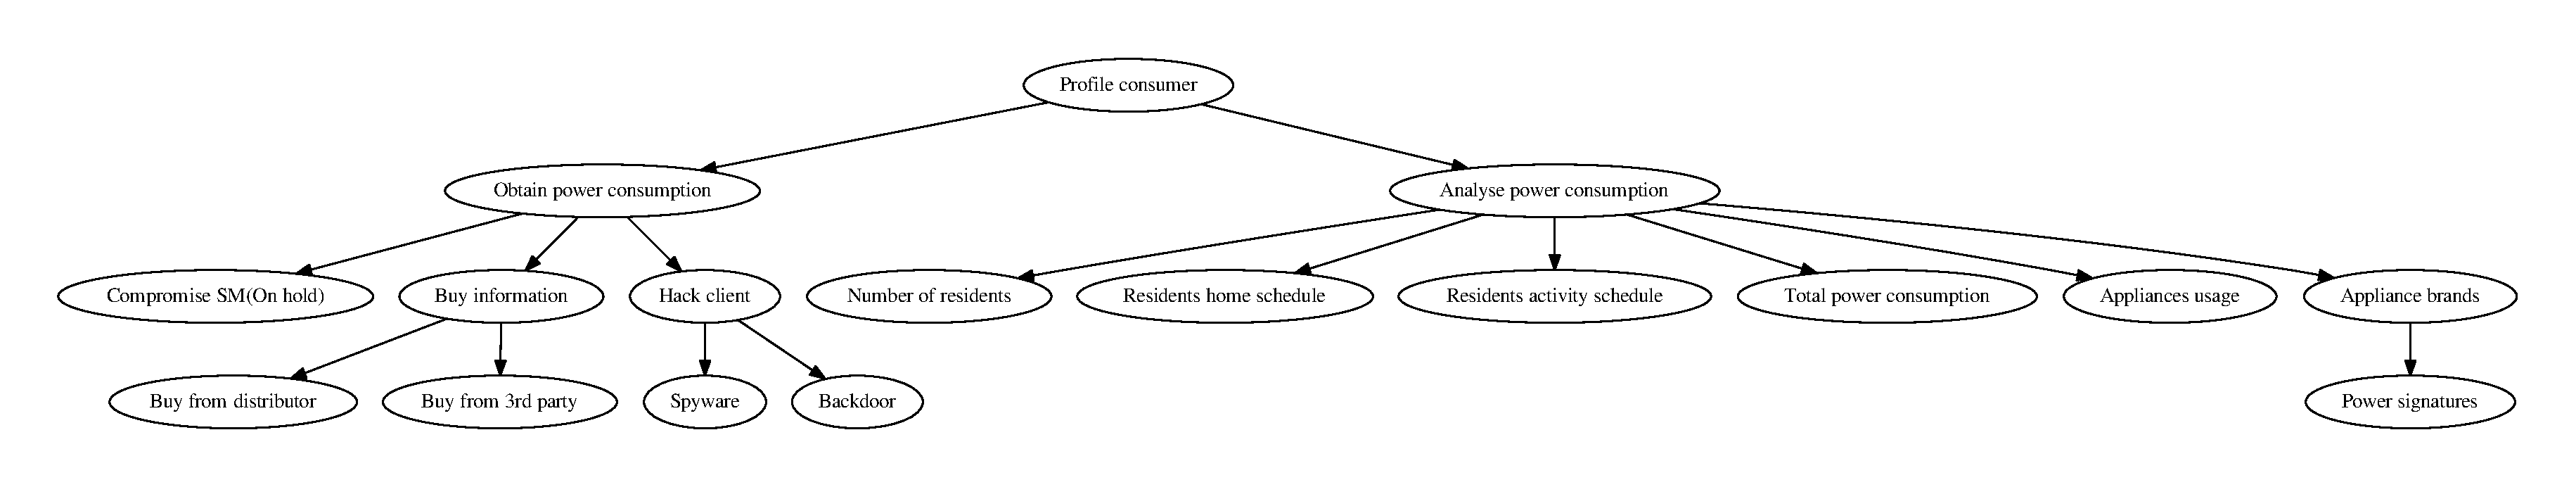
\includegraphics[angle=90, height=\textheight]{graphviz/information_stealing_vs_consumer_tree.pdf}
  \end{center}
  \caption{A information gatherer attacking the consumer by stealing his data.}
  \label{information_stealing_tree}
\end{figure}

\subsection{Obtain power consumption}
In order to analyse the consumption data of the consumer the information gatherer must obtain the consumption first.

\subsubsection{Compromise smart meter}
One way of obtaining this information is to compromise the smart meter of the consumer, either by getting the password for logging into the smart meter or by exploiting a vulnerability in the smart meter implementation. \stefan{måske ville det være rart at kunne referere til buffer overflow her?}

\subsubsection{Compromise client}
Another route for gathering information is through the client connected to the smart meter.

\subsubsection{Buy power consumption}
Another possibility is to buy the information either from someone who has gained access to it or directly from the consumer.
When buying from the consumer social engineering can be used to convince the costumer to sell his data either cheap or against his will.

\subsection{Analyse power consumption}
After gaining access to the smart meter and the consumption data there are many things that can be revealed about the household and the consumers activities and appliances.
See \cref{smart_meter_privacy} to see an example of how the consumption data could be used to reveal this information.
